\documentclass[11pt]{article}
%\renewcommand{\thesection}{\Roman{section}}  %zmiana section na rzymskie
\usepackage[utf8]{inputenc}
\usepackage[OT4]{polski}
\usepackage{tabularx}
\usepackage[margin=60pt]{geometry}
\usepackage{amsmath}
\usepackage{amsfonts}
\usepackage{listings} 
\usepackage[usenames,dvipsnames,table,xcdraw]{xcolor}
\usepackage{array}
\usepackage{sidecap} %do grafik
\usepackage{wrapfig} % j. w.
\usepackage{graphicx} %j.. w.
\usepackage{subfig} %j. w.
\usepackage{booktabs}
\usepackage{longtable}
\usepackage{hyperref}
\usepackage{nicefrac}
\usepackage{multirow}




\begin{document}

\begin{figure} 
\centering
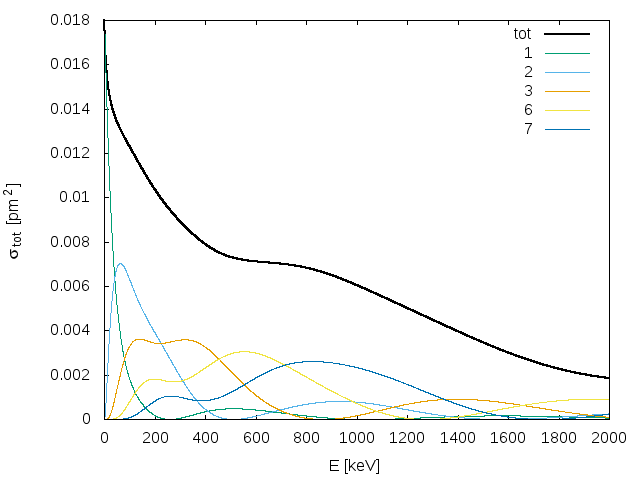
\includegraphics[width=0.8\textwidth]{S+.png}
\caption{}\label{fig:1}
\end{figure}

\begin{figure} 
\centering
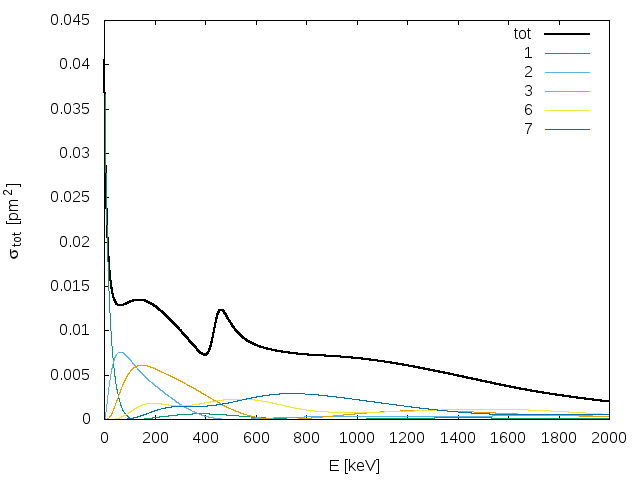
\includegraphics[width=0.8\textwidth]{S-.png}
\caption{}\label{fig:1}
\end{figure}
\begin{figure} 
\centering
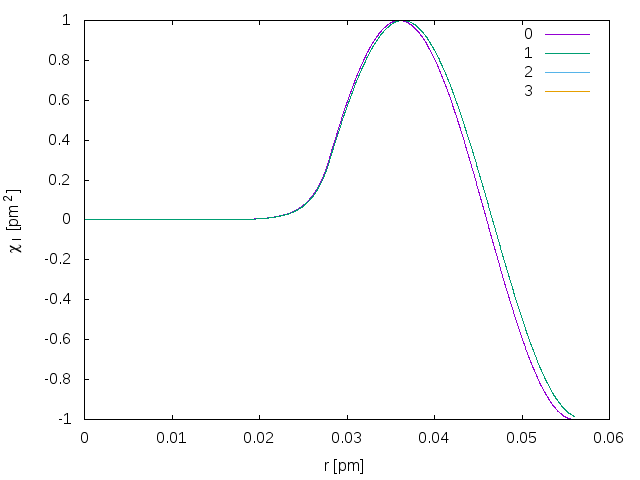
\includegraphics[width=0.8\textwidth]{chi_E10+.png}
\caption{}\label{fig:1}
\end{figure}
\begin{figure} 
\centering
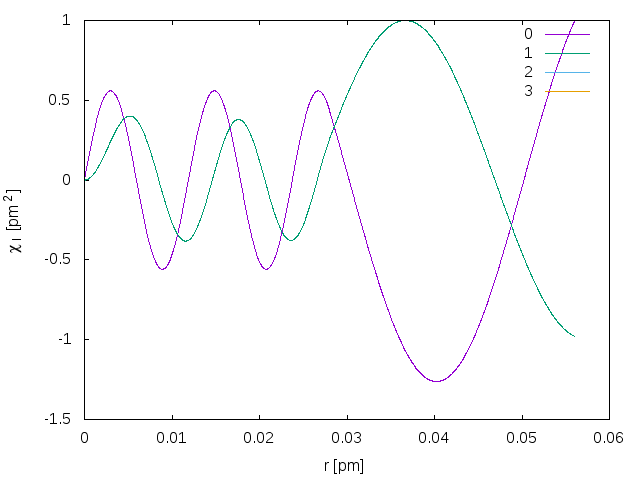
\includegraphics[width=0.8\textwidth]{chi_E10.png}
\caption{}\label{fig:1}
\end{figure}


\end{document}


